% !TEX TS-program = pdflatex
% !TEX encoding = UTF-8 Unicode

% This is a simple template for a LaTeX document using the "article" class.
% See "book", "report", "letter" for other types of document.

\documentclass[20pt]{article} % use larger type; default would be 10pt

\usepackage[utf8]{inputenc} % set input encoding (not needed with XeLaTeX)

%%% Examples of Article customizations
% These packages are optional, depending whether you want the features they provide.
% See the LaTeX Companion or other references for full information.

%%% PAGE DIMENSIONS
\usepackage{geometry} % to change the page dimensions
\geometry{a4paper} % or letterpaper (US) or a5paper or....
% \geometry{margin=2in} % for example, change the margins to 2 inches all round
% \geometry{landscape} % set up the page for landscape
%   read geometry.pdf for detailed page layout information

\usepackage{graphicx} % support the \includegraphics command and options

% \usepackage[parfill]{parskip} % Activate to begin paragraphs with an empty line rather than an indent

%%% PACKAGES
\usepackage{booktabs} % for much better looking tables
\usepackage{array} % for better arrays (eg matrices) in maths
\usepackage{paralist} % very flexible & customisable lists (eg. enumerate/itemize, etc.)
\usepackage{verbatim} % adds environment for commenting out blocks of text & for better verbatim
%\usepackage{subfig} % make it possible to include more than one captioned figure/table in a single float
\usepackage{mathtools}
\usepackage{graphicx} % supports images in latex
% These packages are all incorporated in the memoir class to one degree or another...

\usepackage{graphicx}
\usepackage{subcaption}

%%% Other stuff
\DeclarePairedDelimiter\ceil{\lceil}{\rceil}
\DeclarePairedDelimiter\floor{\lfloor}{\rfloor}

%%% HEADERS & FOOTERS
\usepackage{fancyhdr} % This should be set AFTER setting up the page geometry
\pagestyle{fancy} % options: empty , plain , fancy
\renewcommand{\headrulewidth}{0pt} % customise the layout...
\lhead{}\chead{}\rhead{}
\lfoot{}\cfoot{\thepage}\rfoot{}

%%% SECTION TITLE APPEARANCE
\usepackage{sectsty}
\allsectionsfont{\sffamily\mdseries\upshape} % (See the fntguide.pdf for font help)
% (This matches ConTeXt defaults)

%%% ToC (table of contents) APPEARANCE
\usepackage[nottoc,notlof,notlot]{tocbibind} % Put the bibliography in the ToC
\usepackage[titles,subfigure]{tocloft} % Alter the style of the Table of Contents
\renewcommand{\cftsecfont}{\rmfamily\mdseries\upshape}
\renewcommand{\cftsecpagefont}{\rmfamily\mdseries\upshape} % No bold!

%%% graphics path
\graphicspath{{./HW5}}

%%% END Article customizations

%%% nice things to keep around

% \noindent\rule{2cm}{0.4pt} %%% puts a small horizontal line
% \mathcal{O} %%% big O notation

%%% The "real" document content comes below...

\title{Algorithms Homework 4}
\author{Liam Dillingham}
%\date{} % Activate to display a given date or no date (if empty),
         % otherwise the current date is printed 

\begin{document}
\maketitle

\section{Question 13.3-2} 
Show the red-black trees that result after successively inserting the keys 41, 38, 31, 12, 19, 8 into an initially empty red-black tree. \\
\noindent\rule{2cm}{0.4pt} \\



\begin{table}
\end{table}


\begin{figure}[!htbp]
  	\centering
   	\begin{subfigure}[p]{0.4\linewidth}
    	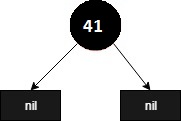
\includegraphics[width=\linewidth]{1.jpg}
     	\caption{Inserting 41}
   	\end{subfigure}
  	\begin{subfigure}[p]{0.4\linewidth}
    	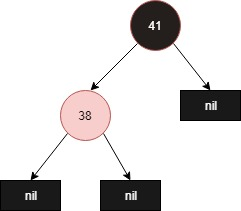
\includegraphics[width=\linewidth]{2.jpg}
    	\caption{Inserting 38}
  	\end{subfigure}

  	\centering
   	\begin{subfigure}[p]{0.4\linewidth}
    	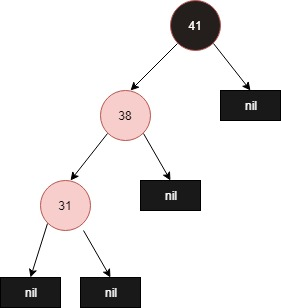
\includegraphics[width=\linewidth]{3-1.jpg}
     	\caption{Inserting 31}
   	\end{subfigure}
  	\begin{subfigure}[p]{0.4\linewidth}
    	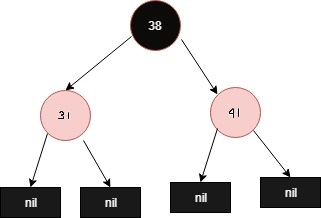
\includegraphics[width=\linewidth]{3-2.jpg}
    	\caption{Re-balancing}
  	\end{subfigure}

   	\begin{subfigure}[p]{0.4\linewidth}
    	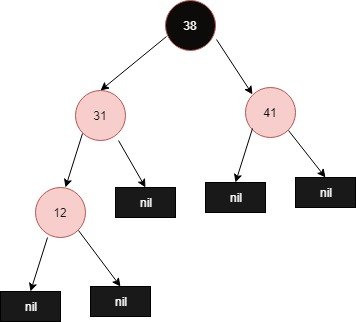
\includegraphics[width=\linewidth]{4-1.jpg}
     	\caption{Inserting 12}
   	\end{subfigure}
  	\begin{subfigure}[p]{0.4\linewidth}
    	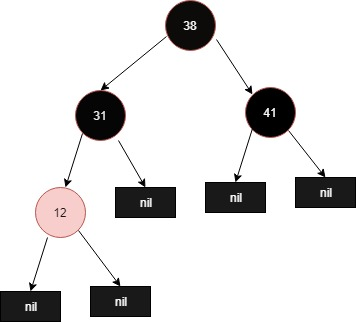
\includegraphics[width=\linewidth]{4-2.jpg}
    	\caption{Re-balancing}
  	\end{subfigure}
\end{figure}
\begin{figure}

   	\begin{subfigure}[p]{0.4\linewidth}
    	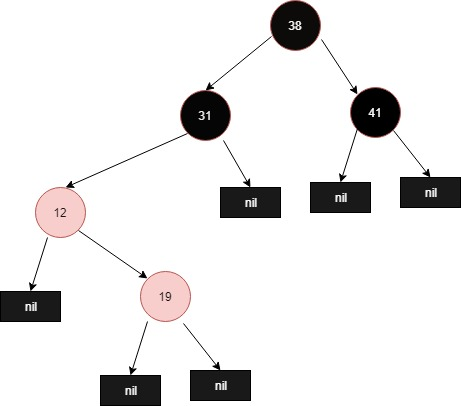
\includegraphics[width=\linewidth]{5-1.jpg}
     	\caption{Inserting 12}
   	\end{subfigure}
  	\begin{subfigure}[p]{0.4\linewidth}
    	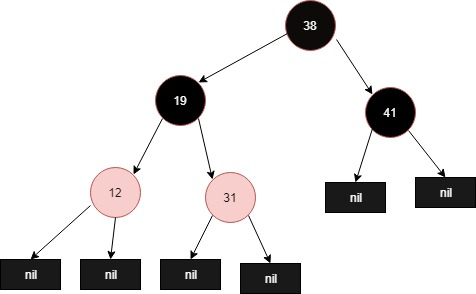
\includegraphics[width=\linewidth]{5-2.jpg}
    	\caption{Re-balancing}
  	\end{subfigure}

   	\begin{subfigure}[p]{0.4\linewidth}
    	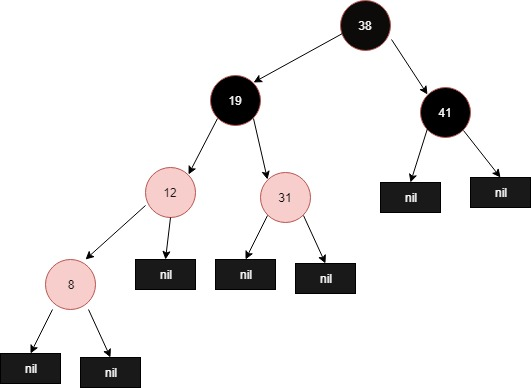
\includegraphics[width=\linewidth]{6-1.jpg}
     	\caption{Inserting 12}
   	\end{subfigure}
  	\begin{subfigure}[p]{0.4\linewidth}
    	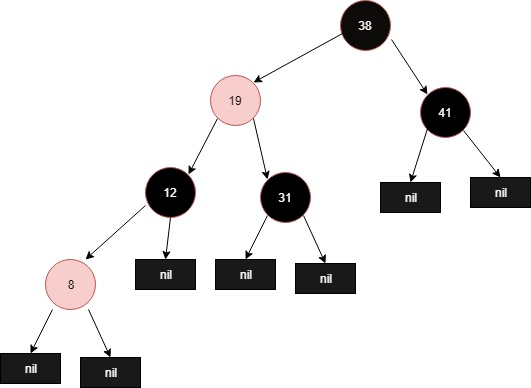
\includegraphics[width=\linewidth]{6-2.jpg}
    	\caption{Re-balancing}
  	\end{subfigure}

\end{figure}

\newpage
\newpage
\newpage
\newpage
\section{Question 13.4-3}
In Exercise 13.3-2, you found the red-black tree that results from successively inserting the keys 41, 38, 31, 12, 19, 8 into an initially empty tree. Now show the red-black trees that result from the successive deletion of the keys in the order 8, 12, 19, 31, 38, 41. \\
\noindent\rule{2cm}{0.4pt} \\

\begin{figure}[!htbp]
  	\centering
   	\begin{subfigure}[p]{0.4\linewidth}
    	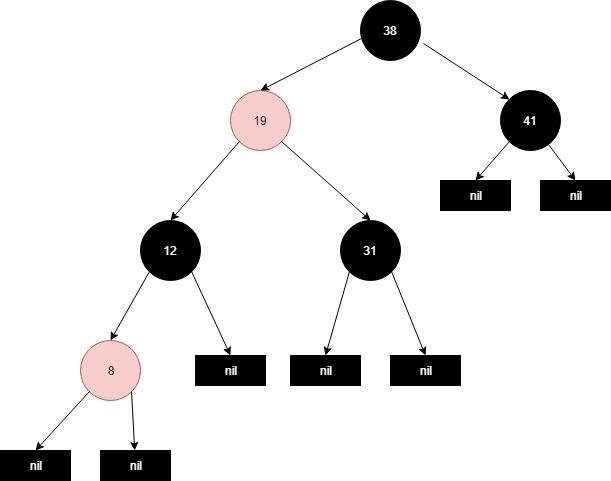
\includegraphics[width=\linewidth]{a1.jpg}
     	\caption{Starting state}
   	\end{subfigure}
  	\begin{subfigure}[p]{0.4\linewidth}
    	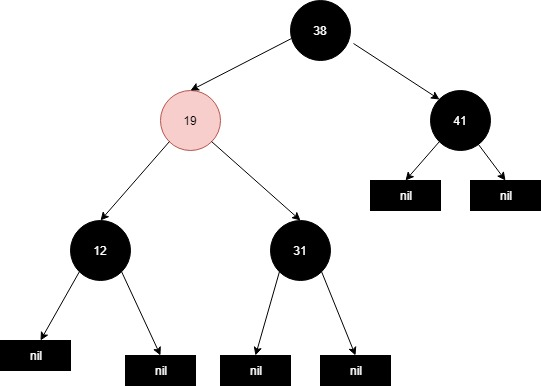
\includegraphics[width=\linewidth]{a2.jpg}
    	\caption{Deleting 8}
  	\end{subfigure}

  	\centering
   	\begin{subfigure}[p]{0.4\linewidth}
    	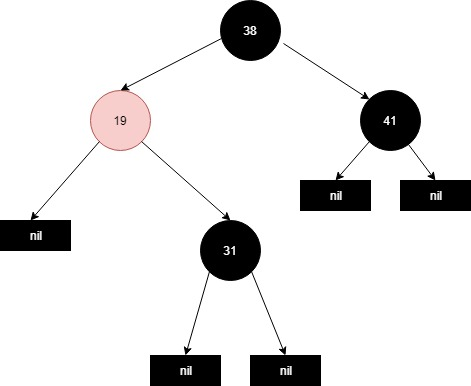
\includegraphics[width=\linewidth]{a3-1.jpg}
     	\caption{Delete 12}
   	\end{subfigure}
  	\begin{subfigure}[p]{0.4\linewidth}
    	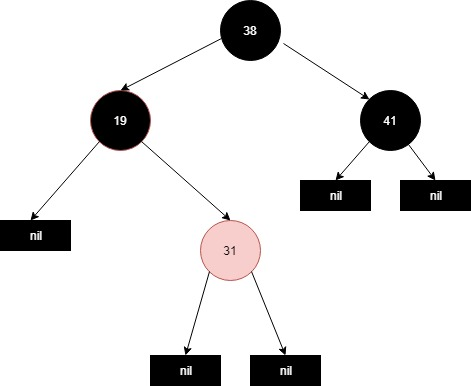
\includegraphics[width=\linewidth]{a3-2.jpg}
    	\caption{Re-coloring}
  	\end{subfigure}

   	\begin{subfigure}[p]{0.4\linewidth}
    	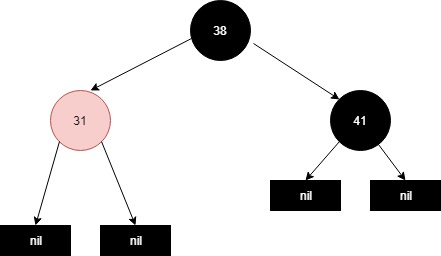
\includegraphics[width=\linewidth]{a4-1.jpg}
     	\caption{Delete 19}
   	\end{subfigure}
  	\begin{subfigure}[p]{0.4\linewidth}
    	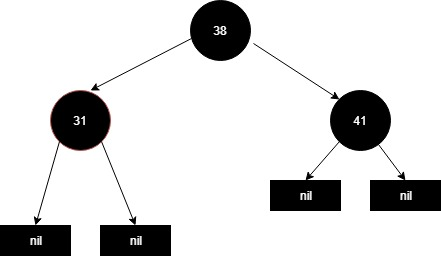
\includegraphics[width=\linewidth]{a4-2.jpg}
    	\caption{Re-color}
  	\end{subfigure}

   	\begin{subfigure}[p]{0.4\linewidth}
    	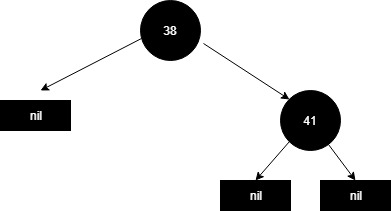
\includegraphics[width=\linewidth]{a5-1.jpg}
     	\caption{Delete 31}
   	\end{subfigure}
  	\begin{subfigure}[p]{0.4\linewidth}
    	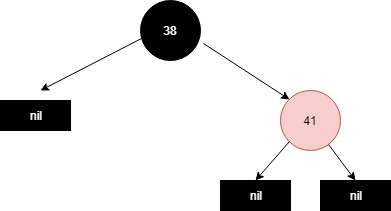
\includegraphics[width=\linewidth]{a5-2.jpg}
    	\caption{Re-color}
  	\end{subfigure}

   	\begin{subfigure}[p]{0.4\linewidth}
    	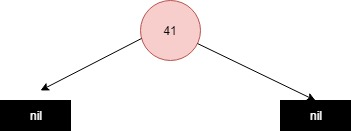
\includegraphics[width=\linewidth]{a6-1.jpg}
     	\caption{Delete 38}
   	\end{subfigure}
  	\begin{subfigure}[p]{0.4\linewidth}
    	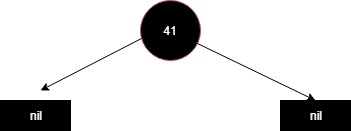
\includegraphics[width=\linewidth]{a6-2.jpg}
    	\caption{Re-color}
  	\end{subfigure}

  	\begin{subfigure}[p]{0.4\linewidth}
    	
\includegraphics[width=\linewidth]{a7.jpg}
    	\caption{Delete 41}
  	\end{subfigure}

\end{figure}

\newpage
\newpage
\newpage
\newpage
\section{Question 14.1-3}
Write a non-recursive version of OS-SELECT. \\
\noindent\rule{2cm}{0.4pt} \\

\begin{verbatim}
OS-SELECT(x, i)
   while x != nil
      r = x.left.size + 1
      if i == r
         return x
      elseif i < r
         x = x.left
      else 
         x = x.right
         i = i - r
\end{verbatim}

with the initial call being OS-SELECT(T.root, i). \\ 
Note that the key change here that causes this function to differ from its recursive counterpart, is that when we meet one of the three conditions (the third being the 'else' clause) we do a reassignment instead of a function call.  If we think about it, a recursive function call is sort of a re-assignment, except we are changing the value of the parameters in the top of a new function call.  Here we are changing the parameters while inside the same call.



\section{Question 14.1-5}
Given an element $x$ in an $n$-node order-statistic tree and a natural number $i$, how can we determine the $i$th successor of $x$ in linear order of the tree in $\mathcal{O}(\lg n)$ time? \\
\noindent\rule{2cm}{0.4pt} \\

determining the $i$th successor of a node x is similar to determining $i$th smallest element, except that we pretend that $x$ is the smallest node in the tree.  So determining the $i$th successor in $x$ is essentially taking the rank of $x$ and adding it to the $i$th smallest element greater than $x$.  So for example, if the rank of $x$ is 4, then finding the 3rd successor of $x$ is equivalent to OS-SELECT(T.root, x.rank + 3) = OS-SELECT(T.root, 7). or to word this generally, we can use the pseudocode function from the book OS-RANK(T,x) and plug it into our OS-SELECT function.
\begin{verbatim}
OS-SELECT(T.root, OS-RANK(T, x) + i)
\end{verbatim}

Note that OS-RANK runs in time $\mathcal{O}(\lg n)$. In addition, OS-SELECT runs in time  $\mathcal{O}(\lg n)$.  Thus the run time of determining the $i$th successor is $\mathcal{O}(\lg n)$ time

\newpage
\section{Question 14.1-6}
Observe that whenever we reference the size attribute of a node in either OS-SELECT or OS-RANK, we use it only to compute a rank.  Accordingly, suppose we store in each node its rank in the subree of which it is the root. Show how to maintain this information during insertion and deletion. (Remember that these two operations can cause rotations). \\
\noindent\rule{2cm}{0.4pt} \\

Once the new node is inserted, we will need to first call PREDECESSOR on our newly inserted node, and set the rank of our new as PREDECESSOR.rank + 1. The we will need to call the SUCCESSOR function for the new node, and on each subsequent node, and increase the rank of each node by 1. \\

Handling the rotations resulting from deletions and insertions is simple; we can simply stick this new logic at the end of the functions.  The modified code for deletions and insertions is shown below:

\begin{verbatim}
RB-Insert(T, z)
   y = T.nil
   x = T.root
	
   while x != T.nil
      y = x
      if z.key < x.key
         x = x.left
      else x = x.right
   z.p = y
   if y == T.nil
      T.root = z
   elseif z.key < y.key
      y.left = z
   else y.right = z
   z.left = T.nil
   z.right = T.nil
   z.color = RED
   RB-INSERT-FIXUP(T,z)

   // Beginning new code
   // Get rank of predecessor and increase the rank of the new node by 1
   z.rank = PREDECESSOR(T, z).rank + 1 

   w = SUCCESSOR(T, z) // Get z's successor
   while w != nil // While there is a successor
      w.rank = w.rank + 1 // increase its rank
      w = SUCCESSOR(T, w) // Get the next successor

\end{verbatim} \\

\newpage
Deletion of a node involves some early book-keeping, but since the rank of the nodes is in linear order, so long as we bookmark the location in the rank list, we can carry on like normal
\begin{verbatim}
RB-DELETE(T,z)
   // Save z's successor
   w = SUCCESSOR(T, z)

   y = z
   y-original-color = y.color
   if z.left == T.nil
      x = z.right
      RB-TRANSPLANT(T, z, z.right)
   elseif z.right == T.nil
      x = z.left
      RB-TRANSPLANT(T, z, z.left)
   else 
      y = TREE-MINIMUM(z.right)
      y-original-color = y.color
      x = y.right
      if y.p == z
         x.p = y
      else
         RB-TRANSPLANT(T, y, y.right)
         y.right = z.right
         y.right.p = y
      RB-TRANSPLANT(T, z, y)
      y.left = z.left
      y.left.p = y
      y.color = z.color
   if y-original-color == BLACK
      RB-DELETE-FIXUP(T, x)

   while w != nil
      w.rank = w.rank - 1
      w = SUCCESSOR(T, w)

\end{verbatim}

\newpage
\section{Question 14.1-7}
Show how to use an order-statistic tree to count the number of inversions (see problem 2-4) in an array of size $n$ in time $\mathcal{O}(n \lg n)$  \\ 
\noindent\rule{2cm}{0.4pt} \\

Problem 2-4 states: \\
Let $A[1..n]$ be an array of $n$ distinct numbers. If $i < j$ and $A[i] > A[j]$, then the pair $(i,j)$ is called an inversion of A. \\ \\

To count the total number of inversion for an array is simple.  For each $j$, count the number of elements greater than $A[j]$ that precede it.  Do this for all $j \in 1..n$, and that is the total number of inversions.  Note that by using an order-statistic tree, we can easily obtain the rank of any element $A[j]$, essentially "sorting" it.  Note also that if an element preceding $j$ is less than $j$, then it is not an inversion. That is, the rank of $j$ is its index minus the number of inversions. $rank(j) = j - NumInversion(j)$. \\

If we re-arrange this equation, we can get $NumInversion(j) = j - rank(j)$. So, by inserting $j$ into the tree, we can find its rank. then we can subtract the rank from $j$, and calculate the number of inversions. Note that both insertion and rank calculation take $\mathcal{O}(\lg n)$ time each. since we have to do this for $n$ elements (from the array), then to calculate the total number of inversions using an order-statistic tree, it will take  $\mathcal{O}(n \lg n)$ time.



\end{document}
